\documentclass[12pt,twoside]{mitthesis}
\usepackage[T1]{fontenc} % font encoding
\PassOptionsToPackage{hyphens}{url}\usepackage{hyperref}
\usepackage[numbers]{natbib}
\usepackage{graphicx, float, color}
\definecolor{mygreen}{RGB}{0, 125, 0}
\newcommand{\review}[1]{{#1}}
\newcommand{\draft}[1]{{#1}}
\newcommand{\wip}[1]{{#1}}
% \newcommand{\review}[1]{{\color{mygreen} #1}}
% \newcommand{\draft}[1]{{\color{blue} #1}}
% \newcommand{\wip}[1]{{\color{red} To do...}}
\begin{document}
\title{Git-Based Platform for Distributed Learning Communities}
\author{Vahid Fazel-Rezai}
\department{Department of Electrical Engineering and Computer Science}
\degree{Master of Engineering in Computer Science and Engineering}
\degreemonth{June}
\degreeyear{2018}
\thesisdate{May 25, 2018}
\supervisor{Philipp Schmidt}{Research Scientist, Director of Media Lab Learning Initiative}
\chairman{Katrina LaCurts}{Chairman, Department Committee on Graduate Theses}
\maketitle
\cleardoublepage
\setcounter{savepage}{\thepage}
\begin{abstractpage}
Instructors use software called learning management systems to administer online courses. Traditionally these digital platforms mimic physical classrooms, but new technology opens up potential for interactions not previously possible. In this thesis, we build a learning management system on top of Git to create a learning environment that encourages collaboration and exploration. We discuss how it was designed following established learning principles, the technical implementation, and the results of a pilot online class, with 100 learners lasting 6 weeks, as part of the Refugee Learning Accelerator. The platform architecture used in this study can be replicated and reused for other online courses with similar goals.
\end{abstractpage}
\cleardoublepage
\section*{Acknowledgments}
I'd like to give thanks to my advisor, Philipp Schmidt, for guiding me in all aspects of this project. I have learned a great deal from working with him and I appreciate his patience and support throughout. I would also like to thank the members of the Learning Initiative, who always pointed me in the right direction.

It was a blessing to be a part of RLA. I am thankful towards Genevieve Barrons, who often defied the bounds of possibility in making the program a huge success, as well as all the instructors and participants in both the online and workshop portions. It was an absolute pleasure to work with everyone. This project would not be possible without a grant from the Open Society Foundation, for which I am also grateful.

\tableofcontents

\newpage
\listoffigures

% \newpage
% \listoftables

\chapter{Introduction}

New education technology, enabled by the Internet, has allowed learners to connect with their instructors and with each other digitally. Pieces of software known as learning management systems take the experience of a classroom online, giving remote learners more access to education and enriching their learning experiences with a variety of technology.

In this thesis I employed Git, a version control technology initially created for collaboration among software developers, as the foundation for an experimental learning platform. The decentralized nature of Git can be utilized to expand interactions beyond replicating a traditional course. New interactions can be designed to balance the benefits of a collective learning experience with those of independent open-ended projects. In this study, I developed a prototype of such a platform, deployed it as part of an online course pilot, and examined the results. With this work, I hope to contribute to lowering the barrier of entry to administer an online course using a Git-based learning platform. The architecture I designed can be built upon in future courses. 

The following sections outline the research methodology of this study. Chapters 2 and 3 cover the theoretical background and other similar projects that were taken as guidance in designing the new platform. Chapter 4 steps through the design and implementation of the platform. Finally, results of a pilot run of using the platform in an online course are presented in Chapter 5. 

\section{Refugee Learning Accelerator}

The development of a Git-based learning platform was part of a larger project called the Refugee Learning Accelerator (RLA). RLA is a program of Media Lab Learning, an initiative of the MIT Media Lab. The goal of the program is to gather and support technologists from the Middle East to develop new education tools for refugee learners. 

\draft{The program ran in three phases from fall of 2017 through spring of 2018. First, interested candidates applied as teams through an open process. Around 100 participants were selected for the first phase of the program, which consisted of a 6-week online course during November and December of 2018. The course operated on a weekly cycle:
\begin{itemize}
\item Challenge materials released every other week introducing a new technology. Teams were asked to design and build a prototype of a solution related to refugee education using that technology.
\item Twice during the week a webinar was conducted where an expert in the field discussed the week's technology and answered questions.
\item Teams were given independence to work as they liked over the course of the week.
\item Teams received qualitative feedback every week from the instructors once a week, at the midpoint and the end of each challenge.
\end{itemize}
The topics chosen for the online course were chatbots, human centered design, and augmented reality (AR). A description of each challenge is included in Appendix A.}

The second phase of the program brought 14 selected teams together for a week-long, in-person workshop in Amman, Jordan. There, teams forged their project ideas through rapid iterations of feedback and field observation. One important goal of the workshop was to foster a supportive community, where members encouraged one another to pursue their projects and share resources.

Following the workshop, teams worked independently to bring their projects to fruition in partnership with local NGOs and with the continued support of the RLA community and Media Lab staff.~\cite{rla}

RLA is the product of the collective effort by members of the Learning Initiative and others passionate about finding creative ways to nurture learning. This included the participants, many of whom worked or studied full-time while participating. The team of instructors included researchers and students from MIT and other affiliated experts. Mentors and speakers from all backgrounds donated their time to assisting teams through the webinars and at the workshop. The program was supported with a grant from the Open Society Foundation, and the development of a learning platform was a key component in the overall operation of its creation and execution.

While one of my goals in building the platform was certainly to support the online course of RLA, I also hoped to explore the possibilities of a Git-based platform more generally. In this way, the online course of RLA served also as a pilot run for the platform in order to evaluate its pros and cons for future adaptations. 

\section{Methodology}

Ultimately the research question I hope to answer in this thesis is: how can Git be used and adapted to support effective online learning communities?

I approached this question in three areas:
\begin{itemize}
\item First, I turned to established theory on digital pedagogy and learning principles to guide the characteristics and ultimately define the interactions of the platform. In particular, I derived these interactions from first principles of learning and the target learning outcomes rather than by attempting to move traditional classroom interactions online.
\item Second, I implemented a technical platform that supports these interactions. The bulk of this work was done before the pilot course, but also includes the technical operation of the course. As much as possible, I relied on third-party software to increase reliability, reproducibility, and familiarity.
\item Third, I used the pilot run to evaluate the platform in practice. In order to gather feedback, I conducted an anonymous online survey among course participants. The survey questions are included in Appendix B. Responses to the survey along with anecdotal evaluation are reported in Chapter 5.
\end{itemize}

The code and course content are all freely available online for use in future iterations of such research.~\cite{rla}

\chapter{Background}

Educational theory and pedagogy comprise a vast field and have been subjects of study since long before the advent of online education. Here we briefly touch on frameworks that I considered for this thesis. 

\section{Traditional Learning Platforms}

An online platform to support learning is not a new concept. A learning management system (LMS) is a tool that helps instructors supervise an online course, and popular commercial LMSs exist such as Blackboard, Moodle, and Canvas. 

A traditional LMS typically provides features including tracking learner grades, file management for assignments and corresponding submissions, and communication mechanisms for instructor announcements or learner questions. These features are often convenient duplicates of the same in-person interactions of traditional classrooms. Furthermore, as LMS is designed to complement traditional classrooms, it usually does not fully encompass the activities of a class, and an all-online course would require a medium of instruction external to the LMS.~\cite{zagalsky2015emergence}

Of note, the issue of learner collaboration, which is often a component of more creative, project-based assignments, is often not fully addressed in traditional LMS platforms. This intersection of collaboration and technology is instead known as computer-supported collaborative work (CSCW), and families of tools exist to support online collaboration. Learners thus would have to take to these external tools to collaborate, depending on the particular assignment.

\section{Foundational Theory}

\subsection{Self-Determination Theory}

A critical underlying assumption of creative learning is that humans have innate desire and ability to pursue their interests, and that the role of the learning environment is to foster the right conditions. This is formalized in self-determination theory (SDT), which delineates three intrinsic pyschological needs:
\begin{itemize}
\item Autonomy: to see oneself as the causal agent of one's life.
\item Relatedness: to interact and connect with others in one's environemnt.
\item Competence: the accumulation of skills and ability to accomplish tasks.
\end{itemize}
SDT suggests that when these three feelings are present, humans are optimally disposed to grow.~\cite{ryan2000self}\cite{selfdetermination2}

The implication of SDT for design of a learning environment is to provide opportunities and encourage learners to be self-driven and motivated to explore their interests. Taking this perspective, not only can the learning environment cultivate ways of providing for the three basic needs prescribed by SDT, but can also channel learners' assumed individual motivation into achieving the desired learning outcomes.~\cite{selfdetermination}\cite{niemiec2009autonomy}

\subsection{Learning Outcomes}

As instructors of RLA, we chose learning outcomes that align with the larger purpose of the RLA program and with consideration of the backgrounds of instructors and participants. 

On a broad level, we borrowed objectives of learning from what is commonly used at the Media Lab and in particular often referenced by Mitch Resnick of the Lifelong Kindergarten group: design creatively, reason systematically, and work collaboratively. These are not specific to RLA, but we referred back to these general principles when defining specific deliverables. In particular, we framed specific objectives in terms of the abilities of learners to think, learn, and work, as opposed to reaching a pre-defined state.~\cite{roleofmaking}

In the case of RLA, we aimed for participants to continue beyond the course in building technologies for refugee learners, which involved outcomes in all three categories:
\begin{itemize}
\item Think creatively about new ways of utilizing technology for learning in unconventional settings.
\item Learn systematically how to find and employ the latest technologies.
\item Work collaboratively with other technologists, NGOs, and instructors to put a solution into practice.
\end{itemize}
The spirit of these outcomes can be found in the choice of challenge topics and deliverables (see Appendix A).

\subsection{The 4 P's}

SDT establishes that learners can be self-driven, and somehow we wanted to cultivate a learning environment that channeled this towards certain broad outcomes. This section fills that gap with a framework for fostering creative learning based on four core components, the four P's of creative learning~\cite{cultivating}\cite{resnick2014give}\cite{creativelearningfuturework}:
\begin{itemize}
\item \textbf{Projects.} Project-based courses forces learners to design creatively and provides space for learners to realize their own vision.
\item \textbf{Peers.} Learning as part of a community not only feeds the relevance component of SDT, but also sets up learners to work collaboratively and build upon each other's work.
\item \textbf{Passion.} SDT posits learners are motivated by the ability to pursue areas of their own interest, which can be built into the learning experience by allowing learners to work on what they care about.
\item \textbf{Play.} In our learning outcomes, there is no preset finished product of learning. The same applies to the process. Allowing learners to tinker and experiment with ideas can help them find the best learning experience for themselves.
\end{itemize}
We centered the design of the learning platform on these 4 P's.

\section{Design Tensions}

Traditional courses emphasize delivering content through lectures, assignments, readings, and evaluations. The 4 P's call for some of the same aspects of traditional courses, but also an aspect of community that must be reconsidered in an online setting. Pulling these together creates tension between ``course'' and ``community'' and requires reconciling opposing characteristics of the learning experience:
\begin{itemize}
\item \textbf{Individual pathways vs shared experiences.} Learners prosper when given independence to really focus on their passions, but would then potentially miss out on experiences on which community can be built. 
\item \textbf{Team work vs solitary work.} Working in a team adds a feeling of belonging, but takes away from the autonomy component of SDT.
\item \textbf{Content vs connection.} Some experiences are great for conveying information that is ultimately needed to learn systematically, but would take away from the unstructured time in which learners can form their own connections.
\end{itemize} 
For each of these tensions, there are clear benefits on both sides. Ideally, a learning experiences mixes and balances both sides of each tension.\cite{learningcreativelearning} 

There are other tensions where our pedagogy stands clearly on one side of the debate:
\begin{itemize}
\item \textbf{Projects vs puzzles.} Projects are open-ended and allow learners to be creative and work along the best path for them. With puzzles, the path to a solution has been decided by the instructor and creativity is limited.
\item \textbf{Open vs closed.} Collaboration and self-driven discovery are easier when course content and others' work is visible to everyone.
\item \textbf{Qualitative feedback vs objective rubric.} A rubric inherently assume that there is a set of checkboxes towards which learners work, again removing creativity and limiting exploration. On the other hand, constructive feedback not only tailors evaluation to the type of work that is best for the learner, but also can be used to encourage further play. Additionally, peer feedback connects learners with each other and enhances the community feeling.
\end{itemize}
We thought about features of the platform and the facilitation of the RLA course along these dimensions.

\chapter{Related Work}

This chapter provides a survey existing technologies and platforms that can can be learned or borrowed from in developing a Git-based learning platform. Git has been applied to many fields, and its application to education has recently come under study by researchers.

\section{Overview of Git}

Git is a technology that is used for online collaboration, particularly in software engineering. Created in 2005 by Linus Torvalds as a tool to support the development of the Linux kernel, Git allows users to each have a local copy of a set of files and sync between their copy and a central server in a coordinated fashion. Git is also a version control system, hence allowing users to backtrack changes or split into multiple branches of work from the same starting state.~\cite{githistory}

Git is used as a command line tool, in which users type text commands to perform the desired git actions, but there are also graphical interfaces available which serve as a wrapper and replacement for the command line. On top of Git, hosting services such as Github, GitLab, and Bitbucket provide a range of features that are as integral to some workflows as Git itself.~\cite{githosting}

Overall, the benefit of Git derives from its powerful capabilities as a collaboration tool, but comes with the cost of an upfront time investment to learn its operation.

\section{Communities of Practice}

A community of practice consists of a group of people, a common interest that they share, and interactions or activities where the group acts on their interest. Members of the community learn from each other and improve their practice. Software development is an example of a community of practice, and Git was created to address the issue of collaboration on code in such a community.~\cite{teachingdigital}

\draft{Git has gone on to prove useful in other communities of practice and has been adapted for collaboration in areas other than code.~\cite{sevenwaysgit} The community of an online course can itself be seen as a community of practice, so other applications of Git may bear lessons on how to adapt it for learning.}

\section{Other Uses of Git}

\draft{
While Git was initially created for and is actively used by the software development community, its application has spread to many other use cases. Here are several of these, and for each the relevant techniques of adapting Git:
\begin{itemize}
\item \textbf{Programming-based courses.} Initially used for collaborating on work, Git is making its way into classrooms as a form of submitting work as well. Instructors may even set up repositories for students for their use or collaboration with teammates.~\cite{whygithubclassroom} Github itself has even added features to streamline this use case.~\cite{githubclassroom} However, note that this is not a LMS and usually is not used as a complete learning platform. Despite this, it is of note that Git hosting platforms can be used a link-able and easily navigable host of information.
\item \textbf{Contest submission.} DevArt by Google ran a contest for which they provided a template repository and submissions were accepted by taking advantage of Github's fork functionality. The template repository was forked over 2000 times.~\cite{devart} Similarly, Mozilla accumulated submissions for its Global Sprint event using the issues feature on Github.~\cite{globalsprint} With this forking mechanism Git can be used to create a submission of work.
\item \textbf{Project management.} Communities of practice centered around a Git repository complete the workflow by using issue tracking (built into Github) and real-time chat services in conjuction with the codebase.~\cite{githubpm} These features are of use in any application of Git, including for discussion or giving feedback in an educational setting.
\item \textbf{Datasets and legislation.} Git hosting platforms have the level of availability and navigation that make them suitable for hosting various collections of information including datasets and pieces of legislation. Here Git serves as a tool to distribute and download content.~\cite{sevenwaysgit}
\item \textbf{Blogging.} The version control aspect of git is often used as a content management system. Github provides support for parsing and serving files in Markdown format as static websites, which makes this even simpler.~\cite{whygithubclassroom}
\item \textbf{Recipes.} A service called Fork the Cookbook allows users can fork, or copy, an existing recipe and tweak it to make it their own. This creates a collaborative and decentralized platform for sharing cooking recipes.~\cite{forkthecookbook}
\item \textbf{Travel logging.} A Github user has a repository for his personal travels, where onlookers can submit suggestions for attractions in a city he is planning to attend by suggesting edits for that particular city's file.~\cite{travellog} Empowering members to contribute to a central file by submitting a suggested edit is a concept that can be taken to other use cases as well.
\end{itemize}
}

\section{Suitability of Git for Learning Platforms}

\draft{While Git was not originally designed as a learning platform, we found in it suitable qualities. Below is a discussion the benefits of git as a tool for fostering educational interactions.

First of all, Git aligns with the design tensions discussed above: 
\begin{itemize}
\item \textbf{Individual pathways vs shared experiences.} Git gives individuals the freedom to take a self-defined path of work by being flexible in how it merges back into the main body of work. Learners can use their preferred tools and platforms, since any file type is supported. At the same time, the project repository acts as a shared space that learners share and can interact with each other in.
\item \textbf{Team work vs solitary work.} Using Git allows learners to work independently on their own time, yet at the same time collaborate with teammates by building on each other's work. After all, its raison d'etre is to be able to build upon each others' work without conflict.
\item \textbf{Content vs connection.} Git can serve as a means of delivering educational content. As discussed in the previous section, Git can also be adapted as the underlying mechanism of a content management system. As a versioning system, Git enables publishing new content, updates, and revisions in a fashion that can be distributed. Popular git hosting websites such as Github and GitLab have built-in support for Markdown-formatted files and support and static web pages. At the same time, learners, can form connections with each other by reviewing each other's commits or suggesting edits to someone else's work. 
\end{itemize}

Git also aligns well with the preferences for the type of experience RLA is designed to be:
\begin{itemize}
\item \textbf{Projects vs puzzles.} Git gives learners room to play, since branches can be made to explore new ideas and unsuccessful changes can be easily reverted.  
\item \textbf{Open vs closed.} By default, everyone's is work openly documented and visible. Commit messages log a complete history of changes.
\item \textbf{Qualitative feedback vs objective rubric.} As a version control system, the currency is in units of iterative work rather than a final deliverable, reinforcing the idea that there is no preset rubric for what is considered good or bad work.
\end{itemize}

Finally, because Git is already widely-used, it is reliable in a technical sense and help material is readily available online for easing adoption. On the flip side, Git's widespread use makes it an important skill. Code collaboration is practically a requirement in the software development industry in particular, and software is increasingly relevant in all industries, so learning Git as part of a participating in course can itself be an additional benefit.~\cite{haaranen2015teaching}}

\chapter{Platform Development}

In this chapter, I walk through the design and implementation of the Git-based platform. 

\section{Design}

In this section I lay out the high-level design for the RLA course. The platform and pedagogy are closely linked, but one does not necessarily imply the other. In other words, while a platform can be built to support a desired pedagogy, the content and facilitation are also critical to achieving it. On the other hand, a particular pedagogical approach may not be possible without a platform that can support it. 

Hence, the design must encompass the whole course, from which the platform design will follow. Though the design targeted the goals of the RLA program, it is intended to be adaptable for other future courses.

\subsection{Balancing Tensions}

\draft{As instructors of RLA, we considered the tensions outlined above in several design decisions, with implications directly in how the course was facilitated and, as a result, the technical requirements of the platform.

\begin{itemize}
\item \textbf{Individual pathways vs shared experiences.}
\begin{itemize}
	\item We allowed learners to apply as teams so that they self-select into groups around work styles, technical interests, and local refugee context. This allows learners to work in teams, but still feel autonomy over who their team is and how they work within their teams.\\ \\The platform, as a result, had to support signing up as predetermined teams.
	\item In webinars, sometimes we asked teams to split up for breakout sessions with smaller groups. This gave learners a chance to meet others outside their team and contribute to the shared experience of the overall course.
\end{itemize}
\item \textbf{Team work vs solitary work.}
\begin{itemize}
	\item Parts of the challenges involved teams agreeing upon a direction and producing a single result, such as identifying a problem to solve or creating a product pitch. Hence, in the platform, we needed a way for learners to collaborate on a single document.
	\item Other parts of the challenges allowed teams to divide work by expertise or interest, such as building a prototype or having different roles in testing with users.
\end{itemize}
\item \textbf{Content vs connection.} 
\begin{itemize}
	\item We wanted learners to have easy access not only to the core course content in which challenges were laid out, but also additional resources they could explore at will. We gathered content and links to resources relevant to each week's challenge and made these available to learners as well. In particular, the platform organized these materials into folders by challenge and clearly indicated which documents were core to the course and which were additional resources.
	\item While this addressed content, we also wanted to address connection. One of the secondary goals of the online course was to foster a community that extended into the later phases of the Accelerator, and communication laid the groundwork for the type of community formed. We allowed for natural and structured opportunities to ask questions and give feedback. We encouraged introductions at the beginning of the course and small talk outside the topic of the challenge was normal. The chat portion of the platform was key to enabling this.
\end{itemize}
\end{itemize}

Along other dimensions we made intentional decisions to promote creative learning:
\begin{itemize}
\item \textbf{Projects vs puzzles.} Each week's challenge was intentionally left open-ended and phrased not as a directive but rather as a question, such as: ``How might we use everyday technologies as learning tools?''
\item \textbf{Open vs closed.} We had to decide how to control the authority of performing actions and the visibility of content. On one hand, we believed that the platform should be as open as possible. On the other hand, we wanted to prevent either intentional or accidental actions that may destroy or hinder other participants' work. Also, we anticipated that sensitive topics could not be expressed without a private way of doing so. Hence, in some places such as edit permissions on the central repository and direct messages we opted for closed interactions. These settings were configured directly into the platform.
\item \textbf{Qualitative feedback vs objective rubric.} We incorporated a weekly review in the form of comments on submissions. Each gave three pieces of feedback following the traffic light approach: one positive (green), one neutral (yellow), and one negative (red). For this feedback, the platform needed support for free-form text comments.
\end{itemize}
}

\subsection{Platform Interactions}

The first interaction learners had with the platform was onboarding. We wanted learners to be able to register for the course as easily as possible, yet still provide basic information to introduce themselves to the rest of the learner community.

After getting set up, most interactions on the platform followed RLA's weekly cycle. In each week of the cycle, content was released at the beginning and learners worked towards a particular milestone by the end of the week. Throughout the week learners could collaborate and participate in seminars. To achieve these requirements, there were four interactions that the core Git-based platform needed to support:
\begin{itemize}
\item \textbf{Content distribution.} New material was posted at the beginning of the week including a description of the week's challenge and targeted milestones. In addition, resources relevant for the week were gathered and provided for learners' reference. This content also sometimes included skeleton code or template documents in which learners could report their progress. These pieces of content required the additional ability of being pulled into learners' working directories.
\item \textbf{Collaboration.} Throughout the week, teams worked together on a single project or codebase in some sort of team work space. 
\item \textbf{Submission.} At the end of the week, learners needed a mechanism to put together a package representing the state of their work on which to receive feedback. We also encouraged learners to use these submissions as a resource to learn from other learners' approach to the challenge.
\item \textbf{Feedback.} We believe frequent personalized feedback can be helpful to learners and also cultivates a culture of collaboration. Hence we wanted the platform to provide an interface where a reviewer can easily peruse a learner's work and leave comments. 
\end{itemize}
Note that all these interactions have similarity in structure with feature development and code review used in software engineering, so we utilized corresponding features in the Git hosting service.

In addition to managing the course content, we also wanted to support a few additional types of communication:
\begin{itemize}
\item For seminars, we needed a way to broadcast video to learners. Additionally, we wanted to engage learners to drive the conversation according to their passions and have face-time with their peers.
\item For technical support and other miscellaneous discussion, we wanted to have an open, real-time, group chat. In particular, the group aspect exposed the entire community to conversations as appropriate so that everyone felt included and in-the-know.
\item For showcasing teams' work, especially to parties outside the course, it was ideal to have a static website summarizing the challenges and the progress coming out of the course. Anyone could then share the link and in this way feel ownership over their work.
\end{itemize}

\section{Components}

\subsection{Git Hosting Service}

In order to have a group of distributed learners participate in the course using Git, we needed to have an server accessible by the Internet running Git where the content would be hosted. We looked at two of the most popular Git hosting services, Github and GitLab. Both offer a SaaS model where they host Git on their servers and simply provide an interface, as well as a self-hosted version where they provide the software but leave running a server to the customer.

We compared the two in terms of features, branding, and technical performance:

\begin{itemize}
\item \textbf{Features.} The two options had very similar sets of features. Github has organizations, teams, repositories, and pull requests, while GitLab has groups, subgroups, projects, and merge requests. Both expose a webhook for Git commits, allow in-browser editing of files, and can serve hosted files as static websites. Both offer free or discounted private repositories/projects for educational uses. On a few points GitLab had additional features, such as being able to request to join a group and being able to trigger scripts that run before serving static websites.
\item \textbf{Branding.} We took into account what implications the branding of the sites would have for learners. Many software companies use Github to host either all their code or even just their open source projects, and as a result a Github profile feels very much like a professional portfolio. We wanted to make sure learners are comfortable experimenting and making mistakes, and took into consideration that some may feel less inclined to do so if the work would permanently be associated with their professional portfolio. 
\item \textbf{Performance.} We took into consideration the technical reliability of each option. We found that GitLab's SaaS offering, GitLab.com, was often slow to load. For both, a self-hosted instance would include considerable setup and costs to run a server, but would allow customizations such as the domain name. Finally, though both are welcoming homes to open source projects, Gitlab has made the web platform itself open source, whereas Github's is not.
\end{itemize}

For our course, we ended up opting for GitLab, and chose to mitigate performance issues by using a self-hosted instance of the free tier. However, it would certainly be possible to adapt our approach for either GitLab or Github, in the both SaaS and self-hosted models.

\subsection{Chat Service}

To allow the development of a community, we wanted to make communication among learners as well as between learners and instructors as open as possible. GitLab alone, with commit messages and comments on merge requests, did not offer as fluid of a setting as we wanted. We decided to augment GitLab with a team-based chat service where learners could communicate in real time.

We looked at existing cloud messaging services including Slack, Gitter, and Mattermost, all of which have a very similar design. They provide open channels where any user can join and chat, as well as messaging between users and in private groups for more direct communication. We hoped to use these spaces as a forum for discussing ideas, asking each other for help, and even just to meet other learners.

From our options we chose to run a self-hosted instance of Mattermost, largely due to our choice of self-hosted GitLab. Mattermost and GitLab have a built-in integration for authentication and backend configuration. Mattermost is also open source, continuing in our spirit of relying on open source tools.

\subsection{Webinar Platform}

\draft{We wanted to incorporate seminars as a component of our course, and for this we needed a video-streaming platform, ideally also allowing learner interaction. The Learning Initiative at the MIT Media Lab has developed exactly such a platform called Unhangout~\cite{unhangout}, so we used this for our course. An Unhangout session has a main video stream and allows participants to break out into smaller groups in a video conference format. Unhangout is also open source.}

\subsection{Internet Accessibility}

\draft{In order to host the components above, to serve websites, and to run any additional scripts, we required an Internet-accessible server. For addressing this need we looked at cloud computing platforms and domain name registration services. There are many vendors in these markets and we didn't find significant benefits in a particular one over any of the others. We ended up using DigitalOcean for the platform server and Namecheap to register the domain.

We also sought to enable HTTPS secure connections to the platform server. To do so, we utilized Let's Encrypt, a certificate authority that provides free automatically generated certificates.}

\section{Technical Infrastructure}

\draft{In this section I walk through the steps of setting up a platform to meet the needs of the design described above. I assume a technical background, in particular familiarity with Internet architecture and Git. My approach was very much iterative, where the most restrictive components were configured first followed by smaller features within that component.}

\subsection{Deployment}

\draft{First of all, I created a droplet in DigitalOcean, which is essentially a virtual machine that would serve as the platform server, with the following specifications:
\begin{itemize}
	\item The server ran Ubuntu Linux as the operating system.
	\item Following GitLab's recommendation, I allocated 4 GB of RAM initially. Later in the course, as the server supported more programs including Mattermost and static webpages, this had to be increased. To do so, I shut down the server temporarily and rebooted the image on a larger droplet.
	\item I initially allocated 60 GB of disk space. As with the RAM, this had to be increased later in the course, especially when participants were storing augmented reality (AR) projects with graphics in their workspaces on the server.
	\item DigitalOcean provides an option to create the droplet using pre-defined imagines, one of which has an instance of GitLab. I chose this image to streamline installing GitLab. Using a different cloud computing provider without such a feature would alternatively require downloading the source code to the server and compiling on the machine manually.
\end{itemize}

Next, I purchased an easy-to-remember domain name (refugeelearning.site) using Namecheap that I could connect to the platform server. This would serve as the landing page and home of the course. To connect this domain to the platform server, I configured nameservers with with A records, which point a domain to an IP address. In particular, I created subdomains as follows, all of which were connected to the IP address assigned for the platform server:
\begin{itemize}
\item \textbf{*}: The * subdomain indicates the root domain, or the absence of a subdomain. The server was ally configured to redirect requests here to the GitLab subdomain, and later this became the address for the course homepage.
\item \textbf{gitlab}: Initially this was called ``code,'' but was renamed to reduce confusion since we started referring to the GitLab instance simply as ``GitLab.'' This was configured to serve the home page of GitLab.
\item \textbf{mattermost}: Initially this was called ``chat,'' but again was renamed to reduce confusion. This was configured to serve the home page of Mattermost.
\item \textbf{pages}: This was reserved for the possibility of teams wanting to create custom portfolios to serve as their own webpages, but in the end this wasn't realized. Instead, I automatically generated websites for each team based on their submitted work and served them as part of the course homepage at the root domain.
\end{itemize}
This could be equivalently be accomplished either in Namecheap's console or by configuring Namecheap to redirect to DigitalOcean's nameservers and configuring the records in DigitalOcean's console. I chose the second to consolidate all configuration to one console.

On the server's side, GitLab has built-in configuration for nginx, which is a tool that directs how web requests to a server are routed and responded to. While GitLab requires certain settings in the nginx configuration files, it also allows for customization that I later used to add capabilities including HTTPS, static sites, and Mattermost.}

\subsection{Server Configuration}

\draft{Throughout this section, I will cover modifications made to the server through SSH in the command line.

The droplet was created with an instance of GitLab already present, so I then went through the process of configuring individual settings for the instance. This was done by changing variables in a specific Ruby file. GitLab provides comprehensive documentation on this configuraton~\cite{gitlabdocs}, but I touch on a few key settings here:
\begin{itemize}
\item The external URL was set to match the registered domain, so that GitLab would automatically configure nginx to route requests to GitLab properly.
\item Email notifications were enabled. To do so, first I created a GMail account for the course administrators and configured GitLab with the appropriate SMTP authentication details. 
\item Custom nginx configuration was enabled. GitLab autogenerates the main nginx files running on the server, so to insert custom configuration requires pointing GitLab to a file containing the additional configurations.
\item Integrating with additional services such as Mattermost and GitLab Runner, which are discussed in more detail below.
\end{itemize}
I then restarted the GitLab service, which triggered GitLab to update its own configuration files in the background. For each key change, I manually tested the functionality; for example, I triggered a test email notification to my own account and checked my inbox for the email. Additionally, on a couple occasions, users needed their passwords reset or accounts deleted, which was accomplished by applying updates to the underlying database through the command line.

By default, GitLab does not support SSL connections and hence accessing the website via HTTPS would not work. To fix this, I used Let's Encrypt's command line tool to issue certificates for each of the subdomains listed above. This involved inserting nginx configuration that would respond to Let's Encrypt's servers' cryptographic challenges. Once set up, these certificates would be valid until expiration 90 days later. This exceeded the length of the course, but were configured to autorenew when close to expiration anyway. 

At this point, the bare version GitLab was fully functional and could be used via the web interface.

The next large component to set up was Mattermost. As with GitLab, Mattermost is open source and was installed by downloading and running the source code on the platform server. Furthermore, GitLab allowed for integration with Mattermost on the level of the server code. This was accomplished with further adjustments in GitLab's configuration. Other configuration could also be made in this file, including:
\begin{itemize}
\item Setting the external URL to properly route requests to the Mattermost instance.
\item Telling Mattermost to recognize HTTPS connections using the issued certificate.
\item Permissions for Mattermost users to create and delete teams.
\end{itemize}
Mattermost also has a mobile client that can be used to access chat channels through a native mobile app. I tested this using my personal phone and wrote instructions for how learners could download and log in to the client.

The most important result of the integration between GitLab and Mattermost was the shared authentication. That is, a user could create an account on the GitLab instance, and then use the same credentials to log in to the Mattermost instance. This greatly simplified the onboarding process for learners.

Finally, a similar process as for setting up Mattermost was required for setting up GitLab Runner. This is a service separate from GitLab that runs the appropriate scripts to prepare and serve static websites using the files in a GitLab-managed Git repository, among other uses. I downloaded the source code onto the platform server and started the service, then adjusted GitLab's configuration file to properly route requests to the service. An additional step here was to register the instance of GitLab Runner with GitLab through GitLab's web interface. After these steps, GitLab users could use the GitLab web interface to trigger jobs for the GitLab Runner instance to run.}

\subsection{Git Architecture and Content Configuration}

\review{The central proposition of the platform is to use Git to support learners' interactions. Here I explore how this can be manifested in Git's specific features.

In particular, Git manages two types of files:
\begin{itemize}
 	\item \textbf{Course content.} Some content is informative and would be best accessed in a single, central location. Other content, such as a submission template, is meant to be acted upon by learners and would ideally be copied and then modified by each team.
 	\item \textbf{Learner work.} On one hand, this work is open-ended and creative, so we want learners to have control over a workspace where they can freely experiment and organize. On the other hand, we wanted a mechanism by which a team can have their work reviewed to receive qualitative feedback from someone else, as well as a way for teams to view each other's work in the line with our goal of having all materials be openly visible.
\end{itemize} 
In these requirements appears again the need to balance between shared experience, a central collection of everyone's work and course content, and individual pathways, giving each team autonomy in their own workspace. We brainstormed a few options of accomplishing this using Git, depending on which Git feature acted as the container of one team's work:
\begin{itemize}
\item \textbf{Organized by folder.} All teams would commit to one shared master branch of a single repository, but in different folders. Each team would work in their own folder and would be able to view others' work in the other folders. General course content would be available in this repository at the root level. Teams can create their own branches as they wish to develop in parallel of their teammates and designate certain branches as ready to receive feedback.\\ \\
The appeal of this approach is its simplicity, but it lacks the ability to enforce permissions preventing one team interfering with another's work.
\item \textbf{Organized by branch.} All teams would commit to different branches of a single repository. This way teams can rebase on master to gain access to new course materials. Though a bit tedious, it is even possible to enforce the appropriate permissions so teams can only push to their own branch. Teams could create additional branches for development and for receiving feedback.\\ \\
The drawback of this method is the disparity between such use of branches and what branches are typically used for. Branches are usually for work-in-progress features or experiments with the intention of eventually merging the branch back. However, here they would be used by teams pursuing totally separate projects in the same place on different branches, which wouldn't make sense to eventually merge. This disparity would potentially confuse users previously familiar with Git and teach improper skills for those who go on to use Git beyond the course.
\item \textbf{Organized by repository.} Each team would work in its own repository, which is created by forking a template repository (inspired by others' use of Git for contest submission). Work from this repository would then be pushed to a subtree within a central course repository.\\ \\
This grants teams absolute freedom within their own repository in terms of permission and usage of branches. A teams is not distracted by seeing other teams' branches on the repository they work in. Additionally, submission snapshots can be created as merge requests to the subtree of the central repository, for which GitLab has a built-in commenting and tagging interface. The downside is that team's work exists in two locations, a development copy in their own repository and a submitted copy in the central repository, which can be more difficult to link together than the separate branches in the previous two approaches.
\end{itemize}
Weighing the pros and cons of each approach, we chose to organize by repository. A key reason was to be able to use the merge request interface for giving feedback, which is shown in Figure~\ref{fig-merge-request}. To mitigate the more complex flow of files between two repositories, we decided to automate the merge request process using custom scripts, which are described in the next section.

Moving forward with the repository-based approach, we created a group in GitLab called RLA with the course's logo and description, so it could be easily found by learners. We also created a corresponding team in Mattermost, which we prepopulated with channels for introductions, technical support, and challenge discussion. We configured permissions so that everything was visible to everyone, but only administrators had permission to create or delete repositories in GitLab.

Within the RLA group, we created two repositories and divided instructor content across them:
\begin{itemize}
	\item \textbf{\texttt{course-central}}. This would contain the core content for each challenge along with additional resources. Under a \texttt{teams} folder, it would also have a subtree for each team, which appears as a folder with all the contents synced from the team's repository. One key file in this repository would be \texttt{participants.json}, a JSON file that would be the source of truth for which learners are registered for the course and for who is on which team. A screenshot of the web interface is shown in Figure~\ref{fig-course-central}.
	\item \textbf{\texttt{team-template}}. This is intended to be forked by teams and would be the method by which new materials would be distributed for teams to work on. For each challenge, teams would pull new material from this template repository into their own copy. Finally, as an added benefit GitLab tracks all the forks of a repository, so teams would not have to additionally register their fork in any way and the subtree in \texttt{course-central} can be generated automatically. A screenshot of the web interface is shown in Figure~\ref{fig-team-template}.
\end{itemize}
A diagram visualizing the flow of content across these repositories is shown in Figure~\ref{fig-diagram}.
}

\begin{figure}[H]
\centering
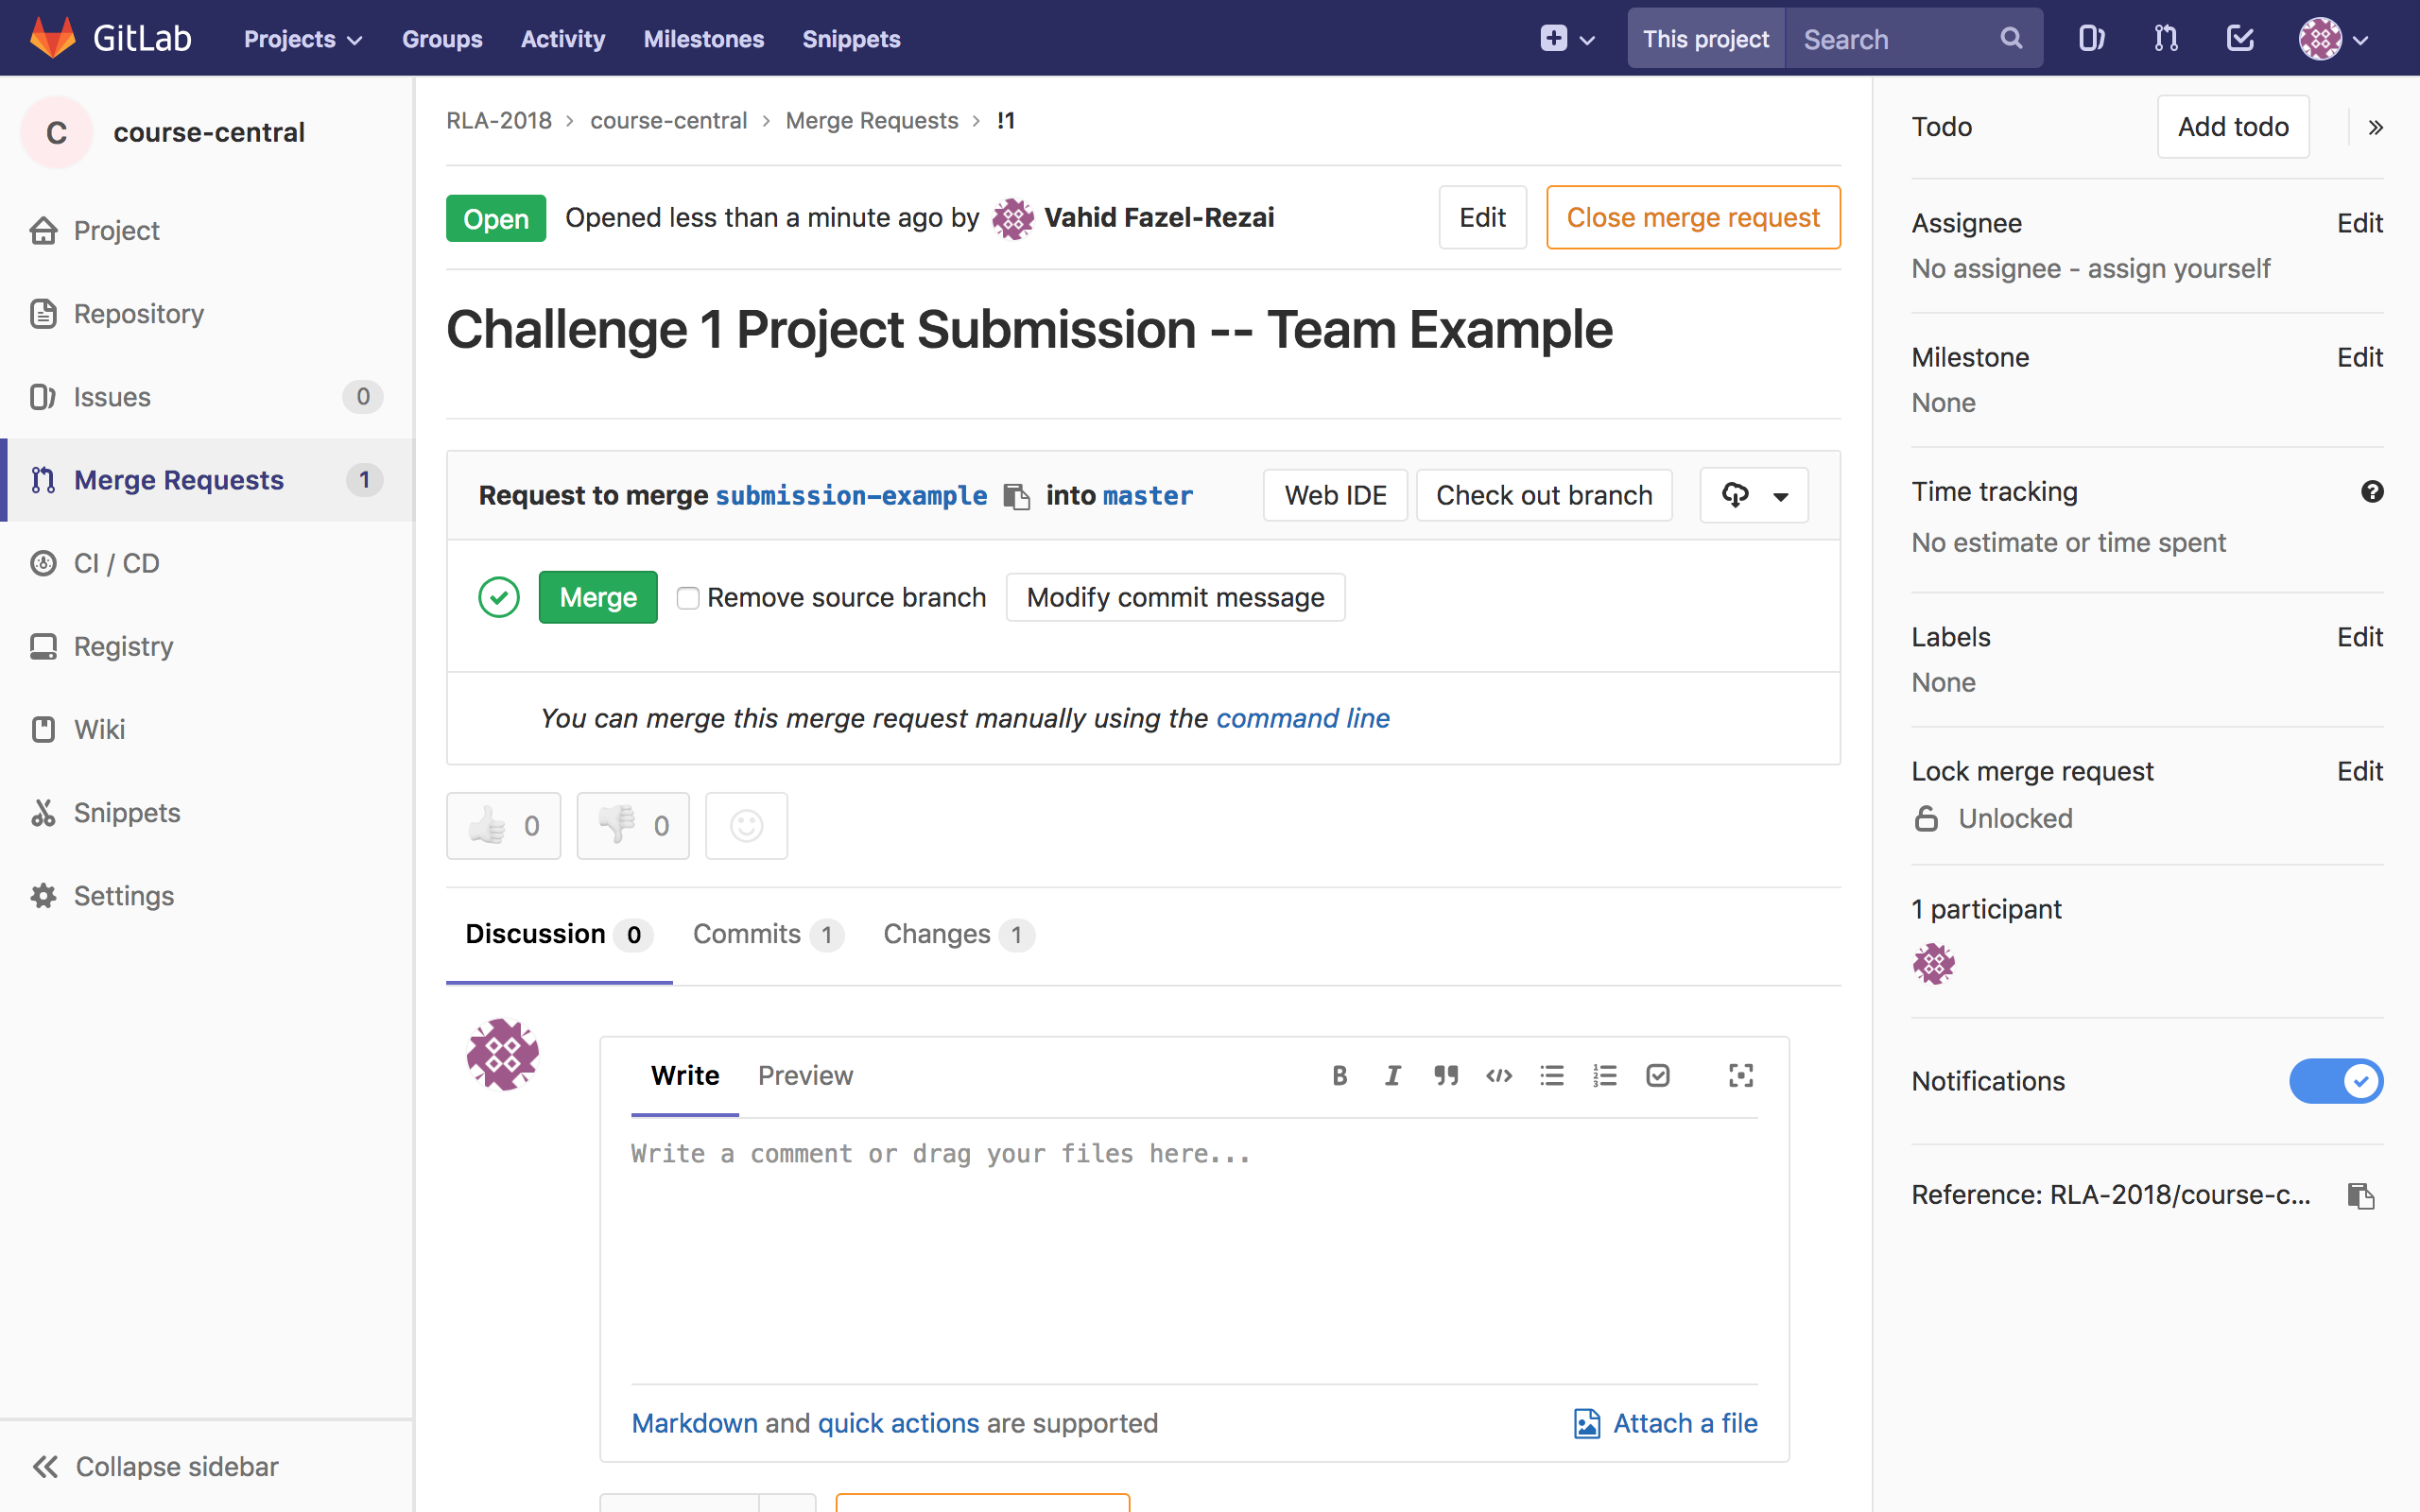
\includegraphics[scale=0.3]{fig-merge-request.png}
\caption{\label{fig-merge-request} The Merge Request interface.}
\end{figure}

\begin{figure}[H]
\centering
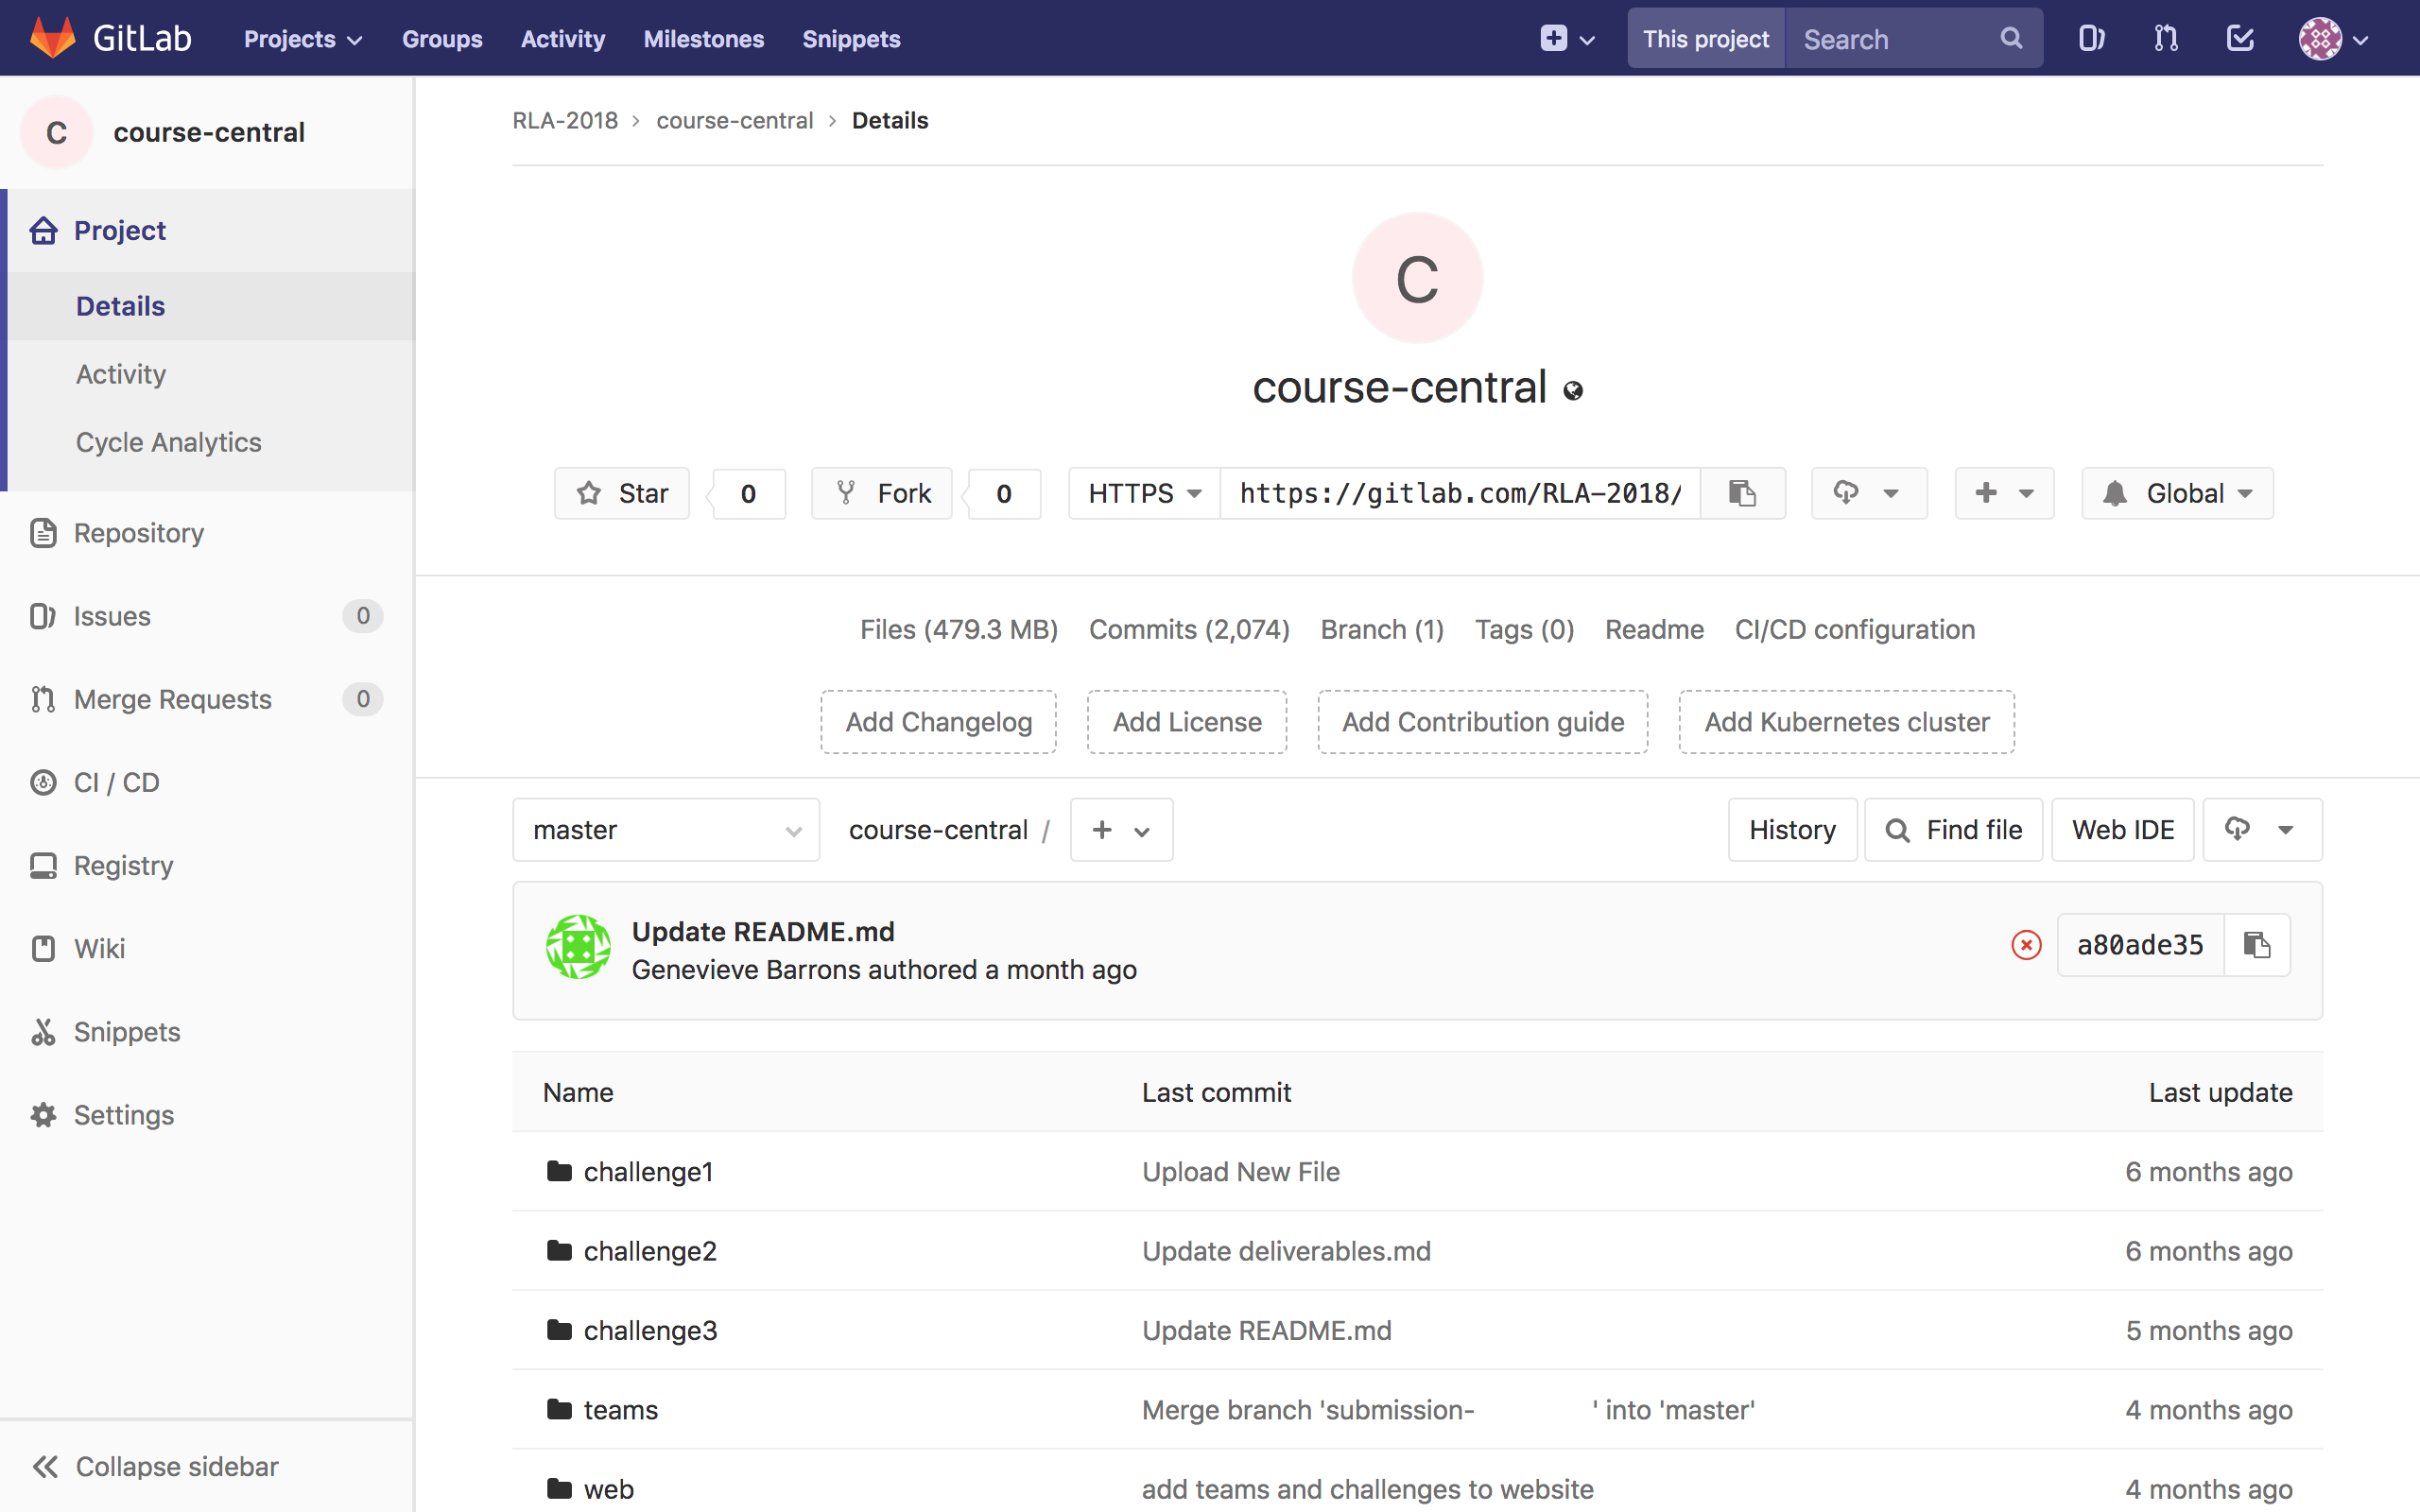
\includegraphics[scale=0.3]{fig-course-central.png}
\caption{\label{fig-course-central} The \texttt{course-central} repository.}
\end{figure}

\begin{figure}[H]
\centering
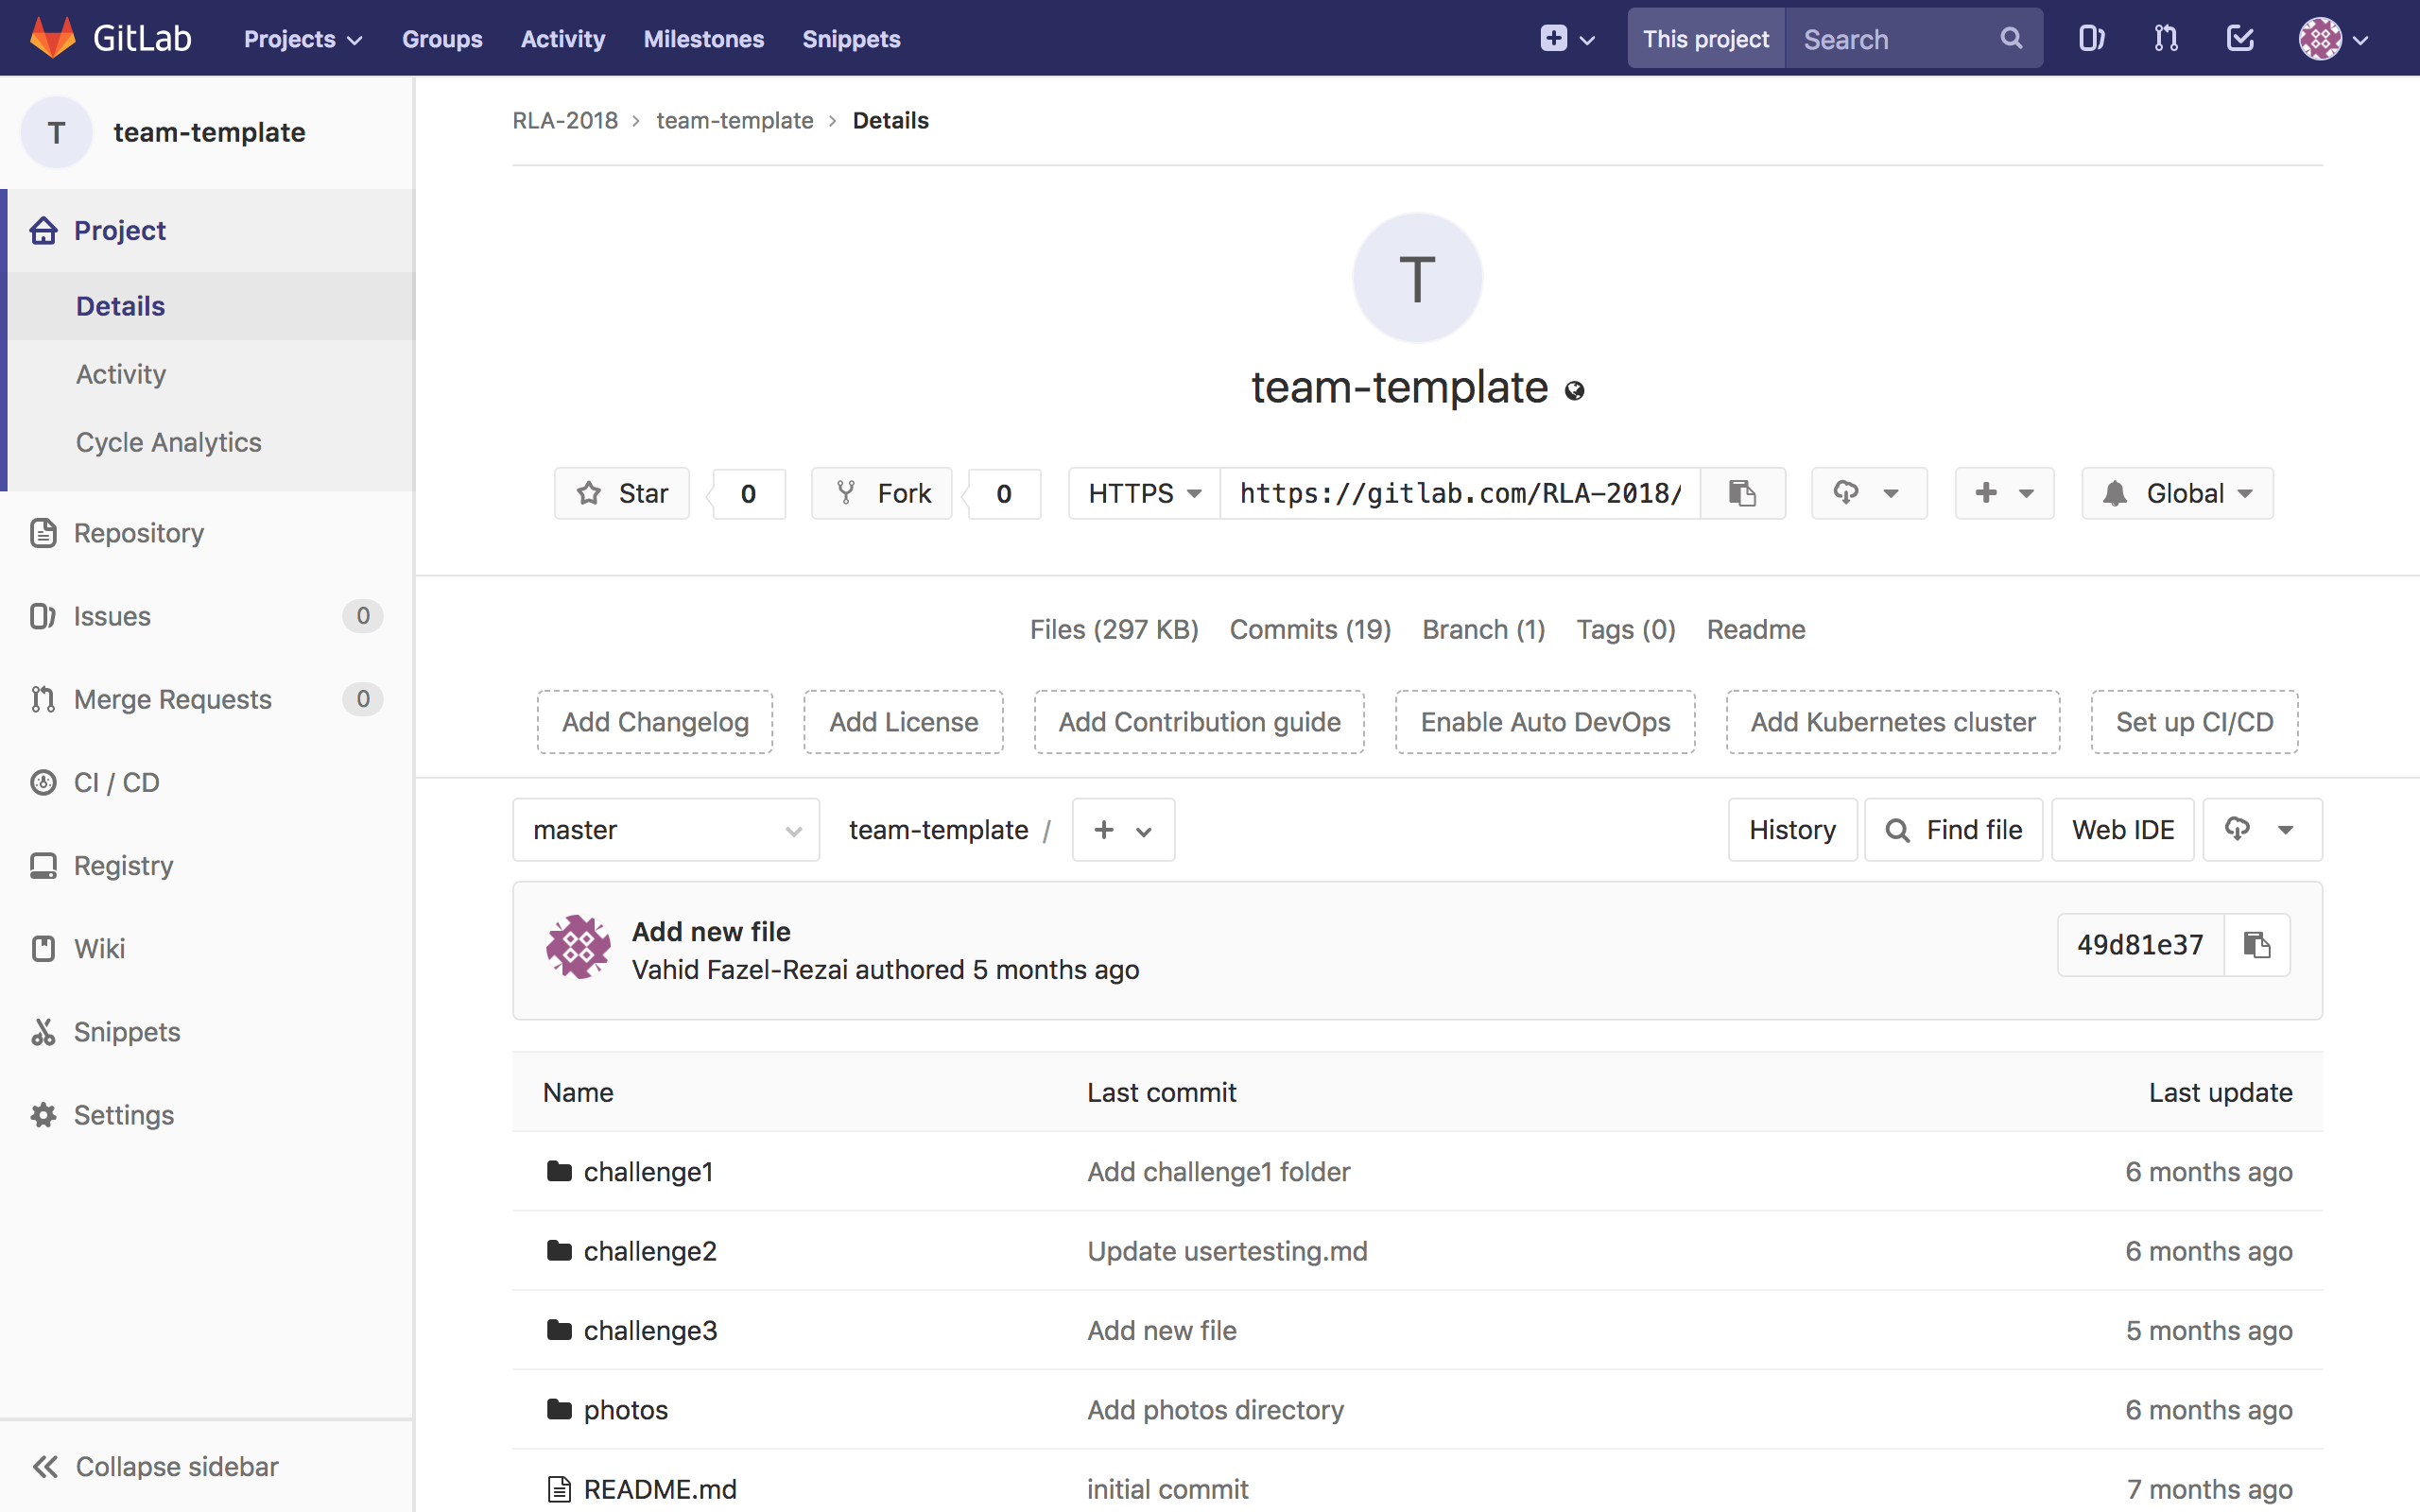
\includegraphics[scale=0.3]{fig-team-template.png}
\caption{\label{fig-team-template} The \texttt{team-template} repository.}
\end{figure}

\begin{figure}[H]
\centering
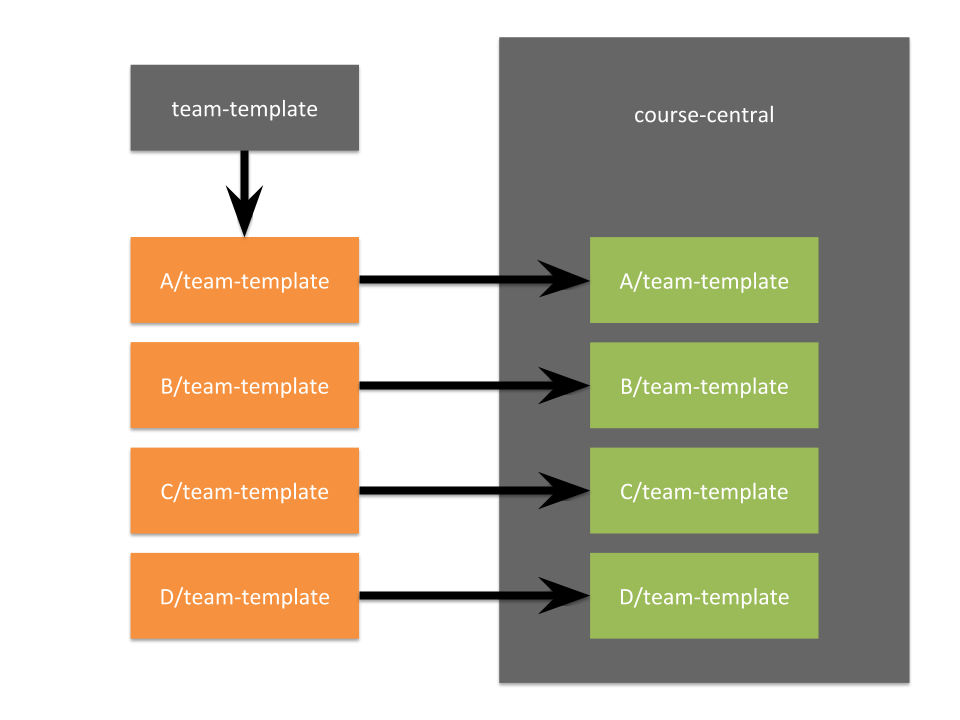
\includegraphics[scale=0.4]{fig-diagram.png}
\caption{\label{fig-diagram} The flow of content. Orange boxes are forks of \texttt{team-template} and green boxes are corresponding subtrees within \texttt{course-central}.}
\end{figure}


\subsection{Custom Scripts and Course Facilitation}

\review{As much as possible, platform-related operations of the course were automated to ease the burden on the instructors. Almost all of these took the form of scripts running on the platform server and using the GitLab API to perform actions on behalf of instructors. More specifically, these actions were associated with the identity of ``RLA Admin,'' represented by a user of that name on GitLab. The scripts were implemented in a combination of Python (for most data manipulation and API calls), Node.js (for continuous scripts that polled an API), and Bash (for running Git commands).

Some scripts were run continually to automatically perform tasks in response to certain events, including:
\begin{itemize}
\item \textbf{Server health check.} Following an incident when a misconfiguration on the platform server left the GitLab site inaccessible, we created a script that would ping the GitLab site every five seconds. In the case that it detected the site was inaccessible, it would send out emails to the instructors alerting them of the problem.
\item \textbf{Analyze team progress.} While the state of each team's work was accessible by everyone, it would sometimes be useful to have an aggregate sense of how many teams had registered themselves in \texttt{participants.json} and for each challenge how many teams had submitted work. Instead of manually navigating and counting on the GitLab website, we wrote a script that could quickly extract a variety of statistics using the GitLab API.
\item \textbf{Approve group membership.} In GitLab, a user must request access to a group from an administrator. Instead of having to wait for an instructor to receive and respond to such a request, we streamlined the learner experience and decided to automatically grant this access (we would still manually review any submissions made to the central repository). To accomplish this, we wrote a script that would poll for pending requests every two seconds and approve them. 
\item \textbf{Create subgroups for teams.} Underneath the RLA group in GitLab, we wanted to create a subgroup with the members of each team. Instead of asking teams or instructors to do this manually, we read team information from \texttt{participants.json} and used the GitLab API to sync this state with membership of subgroups of the RLA group. This was script triggered on every new commit to \texttt{participants.json}.
\end{itemize}
From a learner's perspective, getting started with the course consisted of registering for GitLab, registering themselves in \texttt{participants.json}, and uploading a photo to their team's repository. We expected many learners to be new to Git, so we wrote detailed instructions for accomplishing these tasks to serve the dual purpose of being a first introduction to Git. These instructions are included in Appendix C.

We also utilized scripts for facilitation of the submission process. As laid out above, we allowed teams to do their work in their own repository, but had a collection of all work in \texttt{course-central}. We automated the link between these two with the following scripts:
\begin{itemize}
\item \textbf{Create subtrees.} GitLab tracks forks of each repository, so we ran a script that used a list of forks of \texttt{team-template} to get all the teams' repositories. For each team, it created a branch in the \texttt{course-central} repository that added a subtree linked to the team's repository. The script was idempotent with respect to a given team, so subsequent runs of this script could easily accommodate teams that registered late.
\item \textbf{Create merge request.} At the submission deadline, which we picked to be Sunday at midnight in RLA, we ran a script that created an submission branch on course-central for each team synced with their team repository, and triggered a new merge request from that branch into master. These branches were given a 'submission-' prefix and GitLab permissions were configured to restrict commits to branches with that prefix to just the course administrators. The result in the web interface was a merge request that highlighted the change of a team's workspace since the previous week and allowed anyone to post text comments or tag users.
\item \textbf{Perform merge.} When all the qualitative feedback was completed each week, usually by Wednesday, we used another script to merge and close each merge request. We would then delete all the submission branches and start clean for the following week's submission.
\end{itemize}

In order to publish a new challenge, instructors would take the following steps:
\begin{enumerate}
\item Create a new branch in \texttt{course-central} and progressively add the general informative challenge content. Markdown files can be edited in the browser, other resources can be uploaded or linked. Repeat the same process for adding submission templates to \texttt{team-template}.
\item When ready to release the challenge, merge the challenge branch into master for both \texttt{course-central} and \texttt{team-template}. 
\item Announce the new material by sending learners direct links to relevant materials and notifying them to pull in their team's repository from the template repository.
\end{enumerate}
}

\subsection{Course Webpage}

\review{At any time during the course, \texttt{course-central} contained a collection of all materials generated for and during the course up to that point. By design, most of these materials were contained in Markdown-formatted files, or sometimes in PDF format. Both of these are easy to embed as-is in a website, so we created a course webpage by writing some HTML scaffolding in \texttt{course-central} and setting up GitLab Runner to parse and serve the files in \texttt{course-central} as a static website. The website was arranged with the following pages:
\begin{itemize}
\item \textbf{Homepage and participants.} This was a single page with a description of the course. We had asked teams to upload profile pictures of their members to a particular folder in their team repository. These were then synced to \texttt{course-central} and arranged on the homepage as a directory of all the learners.
\item \textbf{Challenges page.} We gathered all the challenge descriptions and made each of them a tab on one page, so an observer outside the course could quickly get an overview of the course content.
\item \textbf{Team pages.} For each team, we arranged their submission files as tabs on a single page that could be treated as their team portfolio. They could send a link to this page to an observer outside the course to quickly understand what they have produced as part of RLA.
\end{itemize}
We configured the platform server to redirect requests the root domain (refugeelearning.site) to this website. Over the course of the 6 weeks, the website would automatically update with new content as it was committed.
}

\chapter{Results of RLA Pilot}

\review{For six weeks in November and December of 2017, approximately 100 learners participated in an online course using the Git-based learning platform as the first phase of the RLA program. After the course, an optional survey was conducted, the questions of which are included in Appendix B. A total of 11 learners chose to respond to the survey, but since all questions were optional some questions have fewer than 11 answers.

In this chapter I report the experience and results we observed through facilitating the course and the survey responses.}

\section{Git as a Skill}

\review{When asked to what extent they used Git prior to the course, only 1 out of 10 learners indicated at least moderate use Git. All others said they never or rarely used Git prior to the course. We had anticipated this, so we built in several ways to help and encourage learners to learn Git on their own:
\begin{itemize}
\item All learners were aksed to use Git during the onboarding and submission phases. The onboarding instructions, included in Appendix C, give specific Git commands for learners to run.
\item Some teams used Git as their primary collaboration tool.
\item In Mattermost, learners often asked questions when running into errors with Git, and often in answering questions instructors or other learners explained parts of Git.
\end{itemize}
In the survey, 7 out of 10 learners said they found Git useful in their team's collaboration and 8 out of 10 learners said they had at least a basic understanding of Git, even though we provided no formal instruction on Git.}

\section{Submission Process}

\review{From the perspective of the learner, the submission process was entirely automated. Their work appeared in the Merge Requests tab of the \texttt{course-central} repository at the deadline. Over the next couple days, instructors and peers would leave feedback on the merge request, and then it would be merged and closed.

The burden on the learner was to keep their repository up to date, especially at the deadline. In doing this, 4 out of 10 learners reported having issues at some point during the course. One said, ``I believe this was something to do with my local folder and online folder not being updated together. This was down to my inexperience in using git.'' While we tried to simplify the process as much as possible for the learners, Git was still a challenging barrier to overcome.

Another way we tried to simplify the submission process was setting a deadline at which point whatever snapshot was available in teams' repositories would be taken as the submission, although teams who finished after the deadline could notify the instructors and have their submission updated with their latest repository snapshot. The alternative to having a deadline would be to allow teams to trigger the submission themselves, either by creating the merge request themselves or by otherwise triggering the script to run on their repository. When asked whether they would have preferred this alternative, 8 out of 9 learners said no. One commented, ``I believe the deadlines were useful and motivating. If it was a continuous submission then maybe some teams would not have moved on to the next topic easily.'' Another added, ``It is not comfortable knowing access to our work is possible in its draft form.'' While we hadn't factored it into our initial decision. It seemed that conforming to the traditional concept of a deadline resonated with the learners.}

\section{Accessibility of Course Materials}

\review{One of our key principles was to keep course materials, including other teams' work, as open and accessible as possible. 

It seemed that GitLab fit this role well as a content distribution platform, as 9 out of 10 learners reported having no difficulty accessing course materials, with the remaining learner having trouble navigating the submission branches. For informative course content such as challenge descriptions, it seemed like direct links from challenge announcement emails were particularly useful.

Where GitLab exceeded normal content management systems was for the review processing using the merge request interface. In the survey, 10 out of 10 respondents reported being able to view other teams' work and 9 out 10 found this useful. One respondent said, ``It was useful because that allows us to get an idea how others are approaching the same problem that we are working on, and we gained a lot also when others saw our work and gave us feedback.'' 

We also decided to make open and easily accessible the list of participants in the course via the photo gallery on the course homepage. This was possible because we asked for learners to register their team membership and upload their photo as part of onboarding. When asked whether the list of participants was useful, 10 out of 10 participants said yes, with one elaborating, ``It eased to find out the comment came from which group and providing feedback in return.'' This was validation of our hypothesis that, by keeping the course materials open and accessible, learners would make use of it as they need and be self-motivated to act.}

\chapter{Conclusion}

\review{In this thesis I set out to create a new learning platform around the idea that Git as a collaboration tool is in alignment with the 4 P's framework of creative learning. After further exploring relevant theory and other use cases of Git, I worked as part of the RLA instructor team to design a 6-week course that would run on a Git-based online platform. I then implemented a fully functional prototype of the platform largely centered around a self-hosted instance of GitLab. This was ultimately used as the plat the RLA course.

Many of the features of the platform were developed on an as-needed basis in supporting the course, some even while the course was running. This ended up being quite useful, because I could respond directly to feedback and write exactly the scripts that were necessary. Of course, other aspects we had prepared in advance and I am grateful that we did. For example, we chose to create submission templates as Markdown files, which ended up being easy to adapt into team portfolio sites. Overall, developing this platform without a pilot course would have been much more difficult, especially as the course participants were very helpful in their feedback both during and after the course.

In practice, I found that the primary challenge was the knowledge barrier learners had with using Git. Without prior experience, trying to use Git as a component of a larger task could be very frustrating. Perhaps a primer on Git would be a necessary prerequisite for participating with such a platform. 

A secondary and related challenge was navigating the branches and forks of the course's Git architecture. Though more familiarity with Git would partially alleviate this problem, the level of complexity in the Git architecture was a little too high. In the RLA course, not all teams made heavy or even significant use of Git for collaboration, so having a dedicated team repository wasn't the best option for those teams. If I were to redesign the architecture with this in mind, I would choose to have a single repository with a designated folder and a designated branch for each team. The merge request interface worked really well for feedback, so this way a merge request from a team branch into master would still act as a sort of submission. For teams who would want the extra autonomy of having their own dedicated repository, they could set up the same subtree structure that was used in this pilot for themselves without significantly changing the submission workflow.

From learner feedback, having a set submission deadline and an overall weekly cycle seemed to work well. This structure was helpful to balance the open-endedness of the challenge tasks. The structure also eased the load on instructors, reducing the amount of custom attention an instructor needed to give to matters of workflow. Having a predictable seminar and feedback cycle was helpful for those instructors who were writing reviews to plan their schedule.

This pilot also demonstrated how custom scripts can help in facilitating an online course. All of the tasks running as a script were accomplished more easily and faster than manually running Git commands or otherwise completing the task. On the technical side, I believe the greatest opportunity for contribution lies in this area. A production-level, seasoned toolkit for instructors would help Git-based online learning platforms rival traditional LMS.

Finally, creating a course environment that was decentralized, project-focused, and self-driven significantly contributed to creating a friendly community that was enhanced in later stages of the RLA program. In many instances, giving a participant access to information and resources resulted in the participant not only benefiting from it in an unintended way, but also sharing that with other participants. Some of this happened on Mattermost, some within teams, some in the seminar breakouts, and some in the feedback comments. In all cases, openness contributed to participants' learning. In my view, the course served as reinforcement of the frameworks based on which it was designed.}

\appendix

\chapter{RLA Challenge Descriptions}

The online course was divided into three challenges, each of which had two sets of deliverables (one for each week). Here we provide brief descriptions of these. More information as well as various resources related to the topics of each challenge is available online.~\cite{rla} All content was developed by members of the MIT Media Lab Learning Initiative unless otherwise noted.

\begin{enumerate}
\item \textbf{Challenge 1 - chatbots:} How might we use chatbots to support refugee learners inside or outside of the classroom? 
\begin{itemize}
\item Describe your concept for a chatbot in one or two paragraphs. Use visuals (mockups, diagrams) if possible. It is important to be as specific as possible while mapping out the scope of the project as this will greatly influence implementation and the tools to use. Answer the following questions:
\begin{itemize}
\item What problem/ challenge will the chatbot solve? 
\item How will the chatbot solve it? 
\item Who is the primary user and how will the chatbot engage the user?
\item What activity does the chatbot facilitate that would not otherwise be possible? 
\item What challenges do you expect to encounter?
\end{itemize}
\item Demonstrate how your chatbot works. Videos, screenshots or images are encouraged. Add a short description and answer the following questions: 
\begin{itemize}
\item How did you build it? (Platform and technology)
\item What challenges did you face?
\item What aspect of the chatbot do you like best? 
\item What would you different in the future? 
\item Please also add a link to your code!
\end{itemize}
\end{itemize}
\item \textbf{Challenge 2 - human centered design:} How might we use everyday technologies as learning tools?
\begin{itemize}
\item Make an initial prototype. Questions to answer:
\begin{itemize}
\item What solution are you testing? (and why did you choose it?)
\item Submit your prototype (use photos, video, diagrams etc.)
\item Describe the prototype and why you chose this prototyping method. 
\item What did you learn during the prototyping process?
\item Who are your intended users for testing?
\end{itemize}
\item Test it with users. Questions to answer:
\begin{itemize}
\item How did you select your test users? 
\item What was the setting of the test? 
\item What were the main points of feedback you received (share a summary)? 
\item What changes would make to your idea/project based on the feedback?
\item What parts of the Human Centered Design process were new to you?
\item What parts of the Human Centered Design process seemed most useful to you?
\end{itemize}
\end{itemize}
\item \textbf{Challenge 3 - augmented reality (AR):} How might we use Augmented Realtiy (AR) to support refugee language learning outside the classroom?
\begin{itemize}
\item Describe your concept for how low fidelity Augmented Reality could be used to support language learning in one or two paragraphs. Use visuals (mockups, diagrams) if possible. It is important to be as specific as possible while mapping out the scope of the project as this will greatly influence implementation and the tools to use. Answer the following questions:
\begin{itemize}
\item What problem/challenge will the AR experience solve? 
\item How will the AR experience solve it? 
\item Who is the primary user and how will the AR experience engage the user?
\item What hardware does the user need? Is this realistic in the refugee context? 
\item What activity does the AR experience facilitate that would not otherwise be possible? 
\item What challenges do you expect to encounter? 
\end{itemize}
\item Demonstrate how your AR experience works. Videos, screenshots or images are encouraged. Add a short description and answer the following questions: 
\begin{itemize}
\item How did you build it? (Platform and technology)
\item What challenges did you face?
\item What aspect of the AR experience do you like best? 
\item What would you different in the future? 
\item Please also add a link to your code!
\end{itemize}
\end{itemize}
\end{enumerate}

\chapter{RLA Online Course Survey}

The following questions were sent in an email to participants to gather feedback and evaluate how well the platform worked. The survey was anonymous and asked for consent for responses to be used in this research study. A total of 11 participants chose to respond.

\begin{enumerate}
\item Git
\begin{itemize}
\item How much had you used Git before the course?
\item To what extent did you learn Git during the course?
\item How useful would you say knowledge of Git was for collaborating with your team?
\end{itemize}
\item Course materials
\begin{itemize}
\item Did you have any difficulty accessing course materials? If so, what were they?
\item Did you find the course materials helpful in working on your projects? If so, which materials were most helpful?
\end{itemize}
\item Signing up
\begin{itemize}
\item Did everyone on your team submit their own initial sign up on GitLab?
\item How many people on your team used GitLab after the initial sign up? Was there a reason some did not?
\item Did you find it useful to have a list of participants in the course?
\end{itemize}
\item Submission
\begin{itemize}
\item Would you have preferred an automatic, continuous submission (as opposed to your work being snapshot at a set time)?
\item Did you run into any issues in submitting your work? If so, what were they?
\item Were you able to see other team's submitted work? If so, did you find that useful?
\end{itemize}
\item Seminars
\begin{itemize}
\item What were your favorite and least favorite features of the Unhangout platform for seminars?
\item Did you find the seminars useful in ideating for your projects? If so, were any seminars particularly useful?
\item Did you find the seminars useful for the technical side of your projects? If so, were any particularly useful?
\end{itemize}
\item Team
\begin{itemize}
\item How was the technical work distributed among your team?
\item Was your team physically located in the same place?
\end{itemize}
\end{enumerate}

\chapter{RLA Onboarding Instructions}

The sections below are instructions for a new member to get started with the course and complete the first set of tasks.

\section*{Getting started with GitLab and Mattermost}

\begin{enumerate}
\item \textbf{Register a new GitLab account here [linked to GitLab homepage].} We are using a private instance of GitLab specifically for the accelerator, so you will need to create a new account even if you already have one on GitLab.com.
\item \textbf{Join our Mattermost community:}
\begin{itemize}
	\item Go to our Mattermost instance and select \texttt{GitLab} to log in with your new GitLab account. 
	\item You will be asked to join a team. Select RLA. 
\end{itemize}
\item Good job so far. Now it's time to \textbf{Say Hello!} and make some new friends:
\begin{itemize}
	\item Post an introduction in the General channel on Mattermost!
	\item What's your name, where are you from, and what's your Mexican wrestler title?
\end{itemize}
\item \textbf{Join the RLA group on GitLab.} Go back to GitLab. In the top navigation bar, click \texttt{Groups}, then \texttt{Explore public groups}, then \texttt{RLA}, then \texttt{Request Access}. Your request should be approved within a few seconds.
\end{enumerate}

\section*{Register as a team member}

There are two options for how to do this--you may pick whichever you prefer below.

\subsection*{Option 1: Using the GitLab web interface}

\begin{enumerate}
\item Go to here [linked to \texttt{course-central} repository].
\item Under the project navigation bar, click the \texttt{+} button and choose \texttt{New branch} from the dropdown.
\item Write \texttt{register-yourusername} (replacing \texttt{yourusername} with your actual GitLab username) for your branch name.
\item Click \texttt{participants.json} to open the file.
\item Click \texttt{Edit} in the top right and make your edits as described below.
\item Once you're done, press the \texttt{Commit changes} button at the bottom.
\item Navigate back to course-central [linked to \texttt{course-central} repository]. In the project navigation bar, click \texttt{Branches}, then find your branch and click \texttt{Merge Request}.
\item Set \texttt{Assignee} to be \texttt{@vahidfazelrezai}.
\item Click \texttt{Submit merge request}. An instructor will review and merge your request. Once it is merged, you will be added to a subgroup for your team.
\end{enumerate}


\subsection*{Option 2: Using git on the command line}

\begin{enumerate}
\item Run the following in your command line (Terminal on Mac and Command Prompt on Windows), replacing `yourusername` with your actual username:
\begin{itemize}
    \item \texttt{git --version}--if this command fails, you must first install git.
    \item \texttt{git clone https://gitlab.refugeelearning.site/rla/course-central}
    \item \texttt{cd course-central}
    \item \texttt{git checkout -b register-yourusername} (for example: git checkout -b register-*vahidfazelrezai*)
    \item Edit \texttt{participants.json} as described below.
    \item \texttt{git add participants.json}
    \item \texttt{git commit -m 'Register yourusername'}
    \item \texttt{git push origin register-yourusername}
\end{itemize}
\item Go here [linked to \texttt{course-central} repository]. In the project navigation bar, click \texttt{Branches}, then find your branch and click \texttt{Merge Request}.
\item Set \texttt{Assignee} to be \texttt{@vahidfazelrezai}.
\item Click \texttt{Submit merge request}. An instructor will review and merge your request. Once it is merged, you will be added to a subgroup for your team.
\end{enumerate}

\subsection*{How to edit the \texttt{participants.json}}

If you are \textbf{not the primary contact for your team}, you just need to add yourself as a member.

\begin{enumerate}
\item Find your team entry. (If it doesn't exist yet, contact your team's primary contact).
\item Team members need to be separated by \texttt{,}. Add a comma after the last \texttt{\}} in the list of your team members.
\item Starting on the next line after the comma, add your entry. For example, if you were to add to the team above, it would look like:
\end{enumerate}

\begin{verbatim}
{
  "teamName": "team name",
  "members": [
    {
      "name": "PRIMARY CONTACT NAME",
      "username": ":PRIMARY CONTACT GITLAB USERNAME"
    },
    {
      "name": "YOUR NAME",
      "username": "YOUR GITLAB USERNAME"
    }
  ]
}
\end{verbatim}

\textbf{That's it. Well done! Feel free to check in on Mattermost to let us know!}


\section*{Add your photo}

Let's get started. All you need is a image (a photo or any other image to represent you) and to follow these steps:

\begin{enumerate}
\item Navigate to your team's project.
\item Click on the \texttt{photos} directory.
\item Choose an image to upload. \textbf{Important:} Use your GitLab username as the file name, and all lower case, e.g. \texttt{vahidfazelrezai.jpg}. You must rename the file *before* you upload the file.
\item Once you're ready, under the navigation bar, click the \texttt{+} button and choose \texttt{Upload file} from the dropdown.
\item Click \texttt{Upload}.
\end{enumerate}

After you finish these steps there should be a new commit on your project that adds a your photo file. We will automatically pull all photos into a shared class gallery (and share the link very soon!). 

\clearpage
\newpage
\begin{singlespace}
\nocite{*}
\bibliography{sources} 
\bibliographystyle{apa}
\end{singlespace}
\end{document}
